\section{Preliminary Studies}

We have already applied our deadlock freedom check to some 
examples including the classical dining philosopher 
example.
%
Our results show that the method successfully 
and efficiently detects deadlocks when systems are 
deadlock prone.
The method effectively reports deadlock free systems 
where other methods fail to complete analysis. 
Part of the results are published~\cite{FORTE13}. 

\subsection{Dining philosophers}

\begin{figure}
  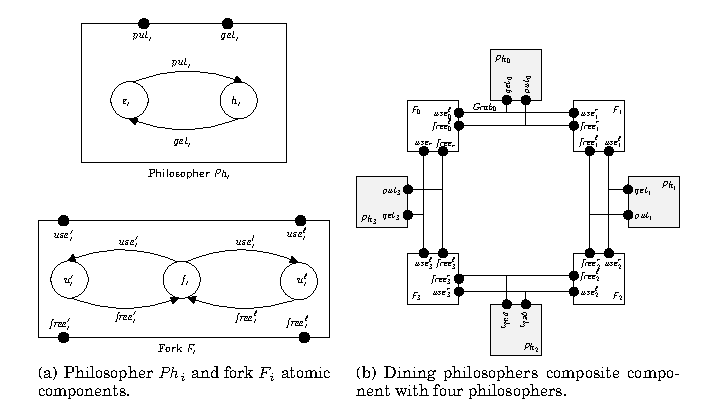
\includegraphics[width=1.1\textwidth]{fig/dining2}
  \caption{Dining philosophers example}\label{fig:dining}
\end{figure}

We consider the traditional dining philosopher problem as depicted in 
Figure~\ref{fig:dining}, which shows $4$ philosophers and $4$ forks modeled in BIP. 

Each philosopher component has $2$ states, and each fork component has $3$ states. 
Thus, the total number of states is $2^n \times 3^n$, for a system
with $n$ philosophers and $n$ forks.

We evaluated our method by increasing $n$ and applying both 
the structural check across all reachable states for a
subsystem and compared against the best configuration 
we could compute with DFinder2 \cite{DFinder2}.
DFinder2 allows for several techniques to be applied. 
The most efficient one is 
the Incremental Positive Mapping (IPM) technique \cite{DFinder2}. 
IPM requires a manual partitioning of the system to exploit its efficiency. 
We applied IPM on all structural partitions and we report on the best result which is consistent 
%(takes less time possibly for hardware related reasons) 
with the results reported in \cite{DFinder2}. 

Table~\ref{bench:dining} shows the results. 
The method outperforms the best performance of 
DFinder2 by several orders of magnitude 
for $n\leq 3,000$. 
The method successfully completed the deadlock freedom 
check for $3,000 \leq n \leq 10,000$ 
in less than one minute, where DFinder2 timed out (~1 Hour). 
%The sole exception being that
%$\LLin$ required $62$ seconds for $n=10,000$. 

\begin{table}
\caption{Benchmarks: Dining Philosopher (seconds or minutes : seconds)}
  \begin{center}
{\normalsize	
\begin{tabular}{| l | l | l |}
\hline
  Size & Method &   D-Finder \\ \hline \hline
$1,000$ &         $0.46 $      & $15$ \\ \hline
$2,000$ &          $1.4 $      & $60$ \\ \hline
$3,000$ &          $2.9 $     & $2:41$ \\ \hline
$4,000$ &          $4.8 $     & $5:37$ \\ \hline
$5,000$ &          $8.3 $     & $12:38$ \\ \hline
$6,000$ &          $13.0 $     & $17:48$ \\ \hline
$7,000$ &          $17.2 $     & $30:18$ \\ \hline
$8,000$ &          $25.6 $     & $-$ \\ \hline
$9,000$ &          $34.1 $    & $-$ \\ \hline
$10,000$ &          $47 $     & $-$ \\ \hline 
\end{tabular}
}
  \end{center}
\label{bench:dining}
\end{table}

We expect that the local deadlock freedom check, along 
with the refinements due to counterexample analysis and 
tighter reachable state space computations will make our 
method more efficient and will allow it to address larger
systems. 


%\subsection{Multi-token based resource scheduler}




